

    Am Anfang jedes neuen Projektes in der Softwareentwicklung muss die Entscheidung getroffen werden, wie qualitativ gut die Software am Ende sein soll.
    Damit sind die Eigenschaften/Funktionalitäten der Software gemeint, die für die Benutzer irrelevant sind, jedoch eine sehr große Bedeutung 
    für das Entwicklungsteam haben.
    
    In der nachfolgenden Tabelle werden die Software, 
    in deren Qualität unterschiedliche Menge an Zeit inverstiert wurde, miteinander verglichen.

    \begin{table}[h!]
        \centering
    \begin{tabular}{ |l|c|c| } 
        \hline
                                                                & viel Zeit & wenig Zeit \\ 
                                                                \hline
        Bugs fixen                                              & schnell       & langsam \\ 
        Neue Funktionalität integrieren                         & schnell       & langsam \\
        Änderungen umsetzen                                     & schnell       & langsam \\ 
        Einarbeitungszeit                                       & gering        & groß \\
        Wahrscheinlichkeit alte Funktionalitäten zu beschädigen & klein       & groß \\
        \hline

       \end{tabular}
       \caption{Vergleich zweier Anwendungen mit viel und wenig inverstierter Zeit in die Architektur}
       \label{tab:compareGoodAndBadArchitecture}
    \end{table}

    Um diese Vorteile (siehe Tabelle \ref{tab:compareGoodAndBadArchitecture}) zu erhalten, muss regelmäßig Zeit in folgende Tätigkeiten inverstiert werden:
    \begin{itemize}
        \item Durchführen von Code Refactoring
        \item Überprüfen der Code Qualität
        \item Durchführen von Code Reviews
        \item Erstellen automatisierte Tests (Unit-, Integration- und Systemtests)
        \item Dokumentation aktualisieren
        \item Technischen Schulden gering halten
    \end{itemize}

    Nicht in jedem Projekt ist das Umsetzen von oben genannten Eigenschaften möglich, 
    da meißt entweder die Zeit oder das Budget oder beides zu gering ist.
    Mit Hilfe folgender Kriterien können einfacher Entscheidung getroffen werden:
    \begin{itemize}
        \item Wann soll die erste Version der Anwendung vorhanden sein.
        \item Wie hoch ist die Anzahl der zur Verfügung stehenden Ressourcen
        \item Wie wahrescheinlich sind die Änderungen und Erweiterungen der Software
        \item Wie kritisch verschiede Probleme und Ausfälle der Software sind 
    \end{itemize}

    In der Abbildung \ref{fig:softQuality} ist zu erkennen, dass auf längerer Distanz eine gute Softwarearchitektur deutlich mehr Funktionalitäten 
    besitzt als eine Software mit schlechter Architektur. Im vorderen Zeitinterval führt allerdings die Software mit der qualitativ schlechteren Architektur.
    \begin{figure}[H]
        \centering
        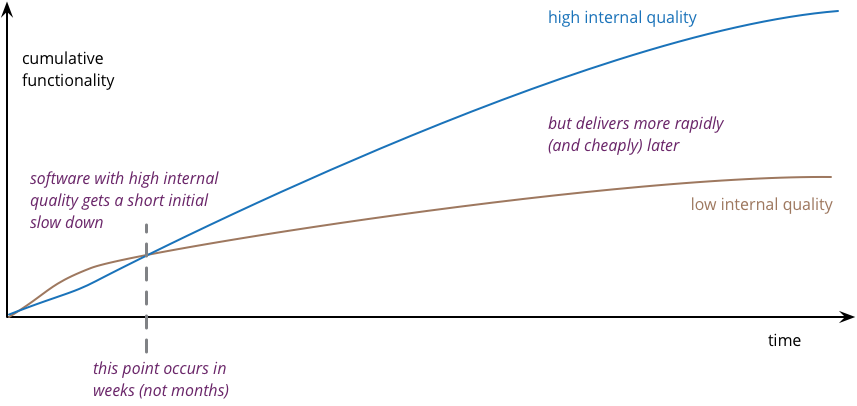
\includegraphics[width=1\textwidth]{./images/QASoftwareCompare.png}
        \caption[Vergleich einer guten und einer schlechten Softwarearchitektur]{Vergleich einer guten und einer schlechten Softwarearchitektur \footnotemark}
        \label{fig:softQuality}
    \end{figure}
    \footnotetext{\url{https://martinfowler.com/bliki/DesignStaminaHypothesis.html}}
    Dieser Verlauf ist bei Projektbegin zu beachten. Es ist nicht von Vorteil bei einem Projekt, 
    für das es nur eine Woche Zeit gibt, viel Zeit für die Architektur einzuplanen, die ohne jeglichen Funktionalitäten mehrere Wochen brauchen wird.

    Wenn das Projekt regelmäßig weiterentwickeln wird, ist es vom Vorteil gleich viel Zeit in der Architektur zu investieren.
